\documentclass{article}
\usepackage{ctex}                               % 显示中文,更改字体
\usepackage{setspace}                           % 调整页行距
\usepackage{geometry}                           % 设置页边距
\usepackage{booktabs}                           % 制作三线表
\usepackage{graphicx}                           % 插入图片
\usepackage{indentfirst}                        % 首行缩进
\usepackage{float}                              % 图片位置
\usepackage{makecell}                           % 处理表格
\usepackage{amsmath}                            % 公式处理
\usepackage{amssymb}                            % 公式处理
\usepackage{titlesec}                           % 标题处理
\usepackage{tikz}                               % 带圈数字
\usepackage{enumerate}                          % 编号排版
\usepackage{appendix}                           % 附录排版
\usepackage{listings}                           % 插入代码
\usepackage{xcolor}                             % 代码颜色
\newcommand*{\circled}[1]{\lower.7ex\hbox{\tikz\draw (0pt, 0pt) circle (.45em) node {\makebox[1em][c]{\small #1}};}}
% 由于自带效果不好,自定义带圈的数字样式
\title{\zihao{-2}自动驾驶中的车辆调头问题\vspace{-2em}}
% 文章标题 且拉进与正文距离 默认 三号
\date{}     % 取消时间显示
\author{}   % 取消作者显示
\renewcommand{\baselinestretch}{1.5}
% 调整行距为1.5倍标准行距
\renewcommand\refname{\ }           
% 把"reference"改成"参考文献"
\renewcommand{\abstractname}{\zihao{3} 摘\ 要\\\vspace{1em}}
% 把“abstract”改成“摘要” 且拉开与正文距离
\geometry{left=3.18cm,right=3.18cm,top=2.54cm,bottom=2.54cm}
% 设置页边距,此处参考word默认间距
\titleformat*{\section}{\zihao{3}\bfseries}
\titleformat*{\subsection}{\zihao{-3}\bfseries}
\titleformat*{\subsubsection}{\zihao{4}\bfseries}
% 三级标题均改变字号,黑体
\titleformat{\paragraph}
{\normalfont\zihao{-4}\bfseries}{\theparagraph}{1em}{}
\titlespacing*{\paragraph}
{0pt}{3.25ex plus 1ex minus .2ex}{1.5ex plus .2ex}
% 设置四级标题 用\paragraph实现
\setcounter{secnumdepth}{4}
% 改变章节编号深度,使得四级标题编号自动生成,如需目录章节深度则使用tocdepth
\lstset{
  language=Matlab,                                          % 代码语言使用的是matlab
  keywordstyle=\color{blue!90}\bfseries,                    % 代码关键字的颜色为蓝色,粗体
  commentstyle=\color{red!20!green!90}\textit,              %  设置代码注释的颜色为绿色
  showstringspaces=false,                                   % 不显示代码字符串中间的空格标记
  stringstyle=\ttfamily,                                    %  代码字符串的特殊格式
  breaklines=true,                                          % 对过长的代码自动换行
  extendedchars=false,                                      % 解决代码跨页时,章节标题,页眉等汉字不显示的问题
  texcl=true}
\lstset{breaklines}                                         % 自动将长的代码行换行排版
\lstset{extendedchars=false}                                % 解决代码跨页时,章节标题,页眉等汉字不显示的问题
\begin{document}
\setlength{\parindent}{2em}
% 首行缩进两字符

\newpage
{\zihao{2}                                                  % 封面
    \qquad
    \\[10ex]
    题目:\underline{\hspace{0.6em} 自动驾驶中的车辆调头问题 \hspace{0.6em}}
    \\[10ex]
    队伍编号:\underline{\qquad \quad 201847100213 \quad \qquad}
    \\[10ex]
    指导老师:\underline{\qquad \qquad \qquad \qquad \qquad \qquad }
}
\thispagestyle{empty}                                       % 本页不生成页码 

\maketitle                                                  % 生成文章题目,作者,时间
\thispagestyle{empty}                                       % 本页不生成页码
\begin{abstract}                                            % 摘要 开始
    {\zihao{-4}                                                 % 摘要 小四
        本文针对无人车自动驾驶时的调头路线轨迹的确定问题,并基于单目标优化模型、差值拟合算法,求出了车辆调头时无障碍物、有障碍物、是否需进行调头情况、是否通过斑马线情况时的轨迹路线。

        对于无障碍物时轨迹路线的确定,首先讨论无人车辆调头的理想路线,在此理想路线上,建立单目标模型进行插值拟合,计算能否得到满足于约束条件的轨迹路线。

        对于是否需要进行调头情况的讨论,在前文的基础上,讨论无人车刚好不需要进行调头的路线,确定临界条件,然后同样建立单目标模型,计算满足于约束条件的轨迹路线。

        对于存在不同障碍物的情况,分别观察和分析障碍物的情况,找出能够行驶的路线,建立多目标模型,计算得出结果判断是否可行。

        对于人行横道的讨论,要考虑不越过和越过两种情况,同时还有障碍物是否存在的情况,当然这与上述只有障碍物的路线相似,只不过多了人行横道这一约束条件,通过建立相关的模型,对可能的路线进行判断,找出能顺利通过的情况。

        对于障碍物移动的情况,考虑提出动态路径规划的技术,根据先验环境模型找出从起点到终点中符合条件的最优或次优路径,涉及的根本问题是环境模型的表达和路径搜寻策略。通过使用人工势场法、启发式搜索算法和基于离散优化的方法等进行求解\\

        \noindent \textbf{关键词:}单目标优化模型 \quad 差值拟合算法 \quad 动态路径规划的技术
        % 局部取消缩进
    }
    \thispagestyle{empty}
    % 本页不生成页码 摘要写的太多 多了一页
\end{abstract}                                              % 摘要 结束
\newpage                                                    % 换页
\setcounter{page}{1}                                        % 文章页码从1开始重新编排
\section{问题重述}                                          % 换页
\subsection{前言}
\zihao{-4}                                                  % 正文小四
自动驾驶是近年人工智能应用的热门研究领域之一,其中调头是自动驾驶中一个非常实际又很有趣的场景。本文所需要解决的问题便是无人驾驶车辆的自动调头轨迹的确定。无人车的轨迹,指的是一条含有位置和时间等信息的曲线,它由一列轨迹点构成,各个轨迹点中应包含位置坐标、方向角、曲率、曲率变化率、速度、加速度及运动到此点时的时间等信息。这里轨迹指的是车身中某一特定点的轨迹,即控制点。

\subsection{相关参数}
假设无人车为四轮乘用车,采用前轮转向后轮驱动; 车身可认为是一个矩
形,车长 5 米,车宽 2 米,轴距 $2.8$ 米; 方向盘最大转角 470,方向盘与前
轮转角的传动比为 16:1(方向盘每转动 $16^{\circ}$, 前轮转动 1),方向盘最大转
速为 $400^{\circ} / \mathrm{s} ;$ 最大油门加速度 $3 \mathrm{~m} / \mathrm{s}^{2}$, 极限杀车加速度-5m/s $^{2}$ 。

\subsection{限制条件}
\noindent 无人车行驶时需要满足以下动力学条件:

\noindent(1)任何点的加速度不得高于最大油门加速度,不得低于极限刹车减速度;

\noindent(2)无人车朝向和方向盘转角都不能突变,轨迹线必须是连续、且切线方向连续,当无人车不是静止时,曲率也必须连续(静止时可以原地打方向,非静止时不能);

\noindent(3)轨迹线的最大曲率应尽量不高于 0.205,禁止高于 0.21;

\noindent(4)按轨迹行驶时,在调头完成之前,无人车车身任何点不得与任何障碍物或者调头区域边界发生碰撞,且与障碍物至少保留一个最小安全距离,一般不小于 30cm。无人车调头轨迹在保证上述条件之外也应具备尽可能舒适的驾乘体感,以及具备尽可能高的通行效率,同时出于规范驾驶的考虑,尽量减少不必要的压车道线行驶。

\subsection{解决问题}
\noindent 问题 1:如图1所示场景,无人车正在最左侧车道准备调头,存在三个对向车道。当无人车身触碰到对向的调头区域边界时,认为调头完成。请阐述控制点位置,解释其理由;基于此建立无人车调头的数学模型,并给出一个合理可行的算法设计,给出调头轨迹。

\begin{figure}[H]% 先尝试能否将照片放在原处(here),如果不能,那么放在页面底部(bottom),最后尝试放在顶部(top) 都不可以采用H强制放在原位
    \centering
    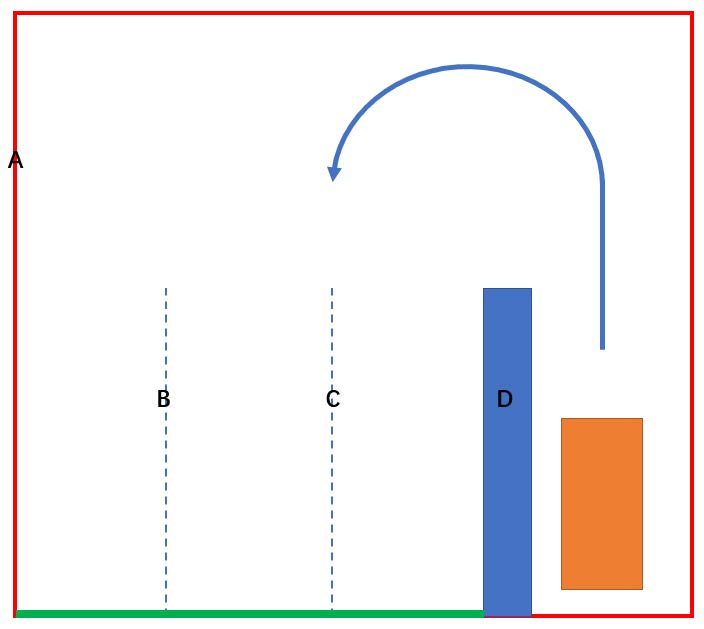
\includegraphics[scale=0.8]{1.jpg}
    \caption{无人车调头场景1}
\end{figure}

问题 2:当调头区域狭窄时,判断什么样的场景下无人车能够在不倒车的情况下完成调头,什么情况需要至少一次倒车才能通过。

\begin{figure}[H]% 先尝试能否将照片放在原处(here),如果不能,那么放在页面底部(bottom),最后尝试放在顶部(top) 都不可以采用H强制放在原位
    \centering
    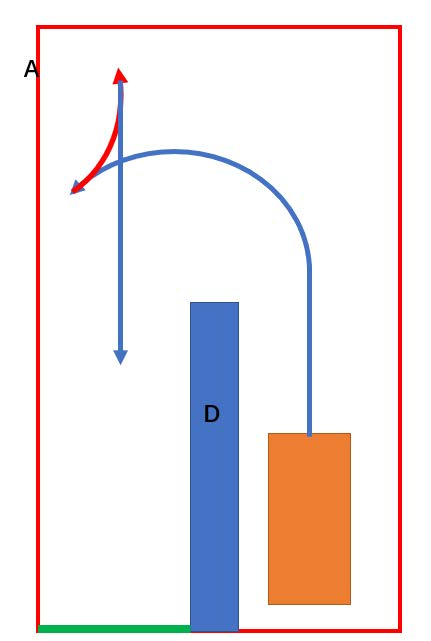
\includegraphics[scale=0.8]{2.jpg}
    \caption{无人车调头场景2}
\end{figure}

问题 3:如图 3 场景,如果道路上还存在其它静止障碍物,当仅存在 F、仅存在 G、或二者都存在时,建立相应的无人车调头的数学模型,给出合理的算法设计,并给出调头轨迹,你的算法应明确如何进行避障?

\begin{figure}[H]% 先尝试能否将照片放在原处(here),如果不能,那么放在页面底部(bottom),最后尝试放在顶部(top) 都不可以采用H强制放在原位
    \centering
    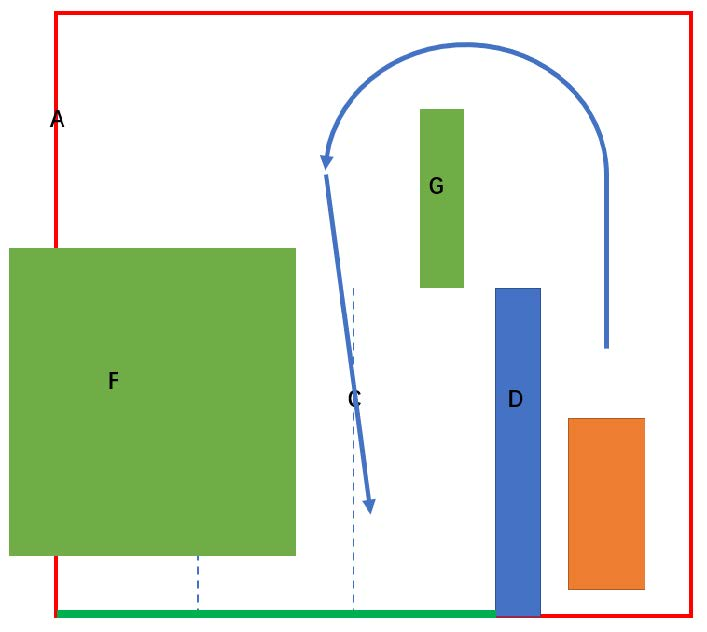
\includegraphics[scale=0.8]{3.jpg}
    \caption{无人车调头场景3}
\end{figure}

问题 4:如果道路上存在人行横道即斑马线E,则无人车需要尽可能在不压人行横道的情况下过,如果无法做到,则需要越过人行横道后再开始调头,禁止骑人行横道调头。建立相应的无人车调头的数学模型,给出合理的算法设计和相应的调头轨迹;当斑马线和障碍物同时存在时(如图5所示),你的模型和算法如何同时满足交规并进行避障绕行?

\vspace{0.5ex}
\begin{figure}[hbt]
    \begin{minipage}[t]{0.5\textwidth}
        \centering
        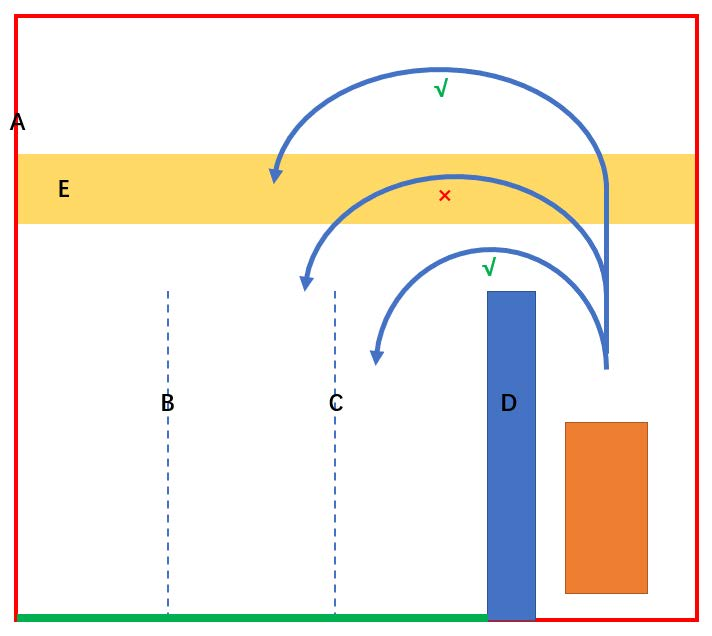
\includegraphics[scale=0.8]{4.jpg}
        \caption{无人车调头场景4}
    \end{minipage}
    \qquad
    \begin{minipage}[t]{0.5\textwidth}
        \centering
        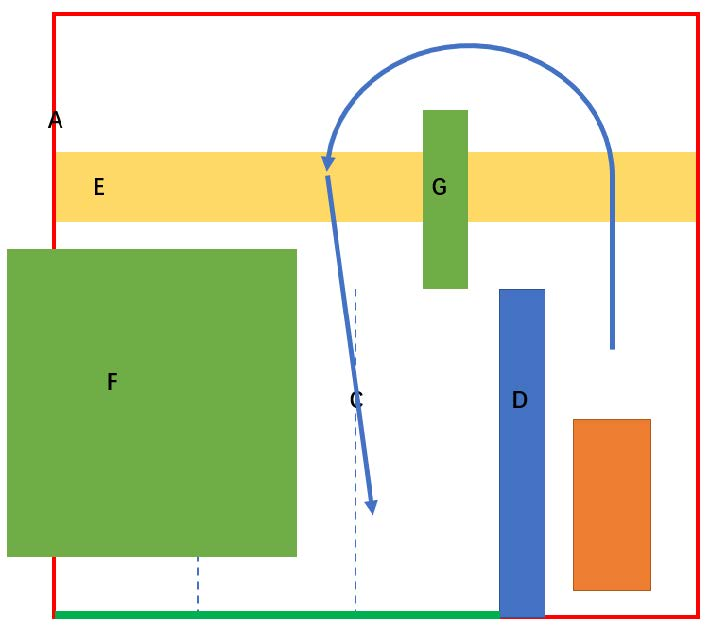
\includegraphics[scale=0.8]{5.jpg}
        \caption{无人车调头场景5}
    \end{minipage}
\end{figure}
\vspace{0.5ex}

问题 5:无人车在实际路况行驶中进行调头时,道路中的障碍物通常是处于移动状态,如对向来车等,针对图3和图5的两种场景,假设图中标识的障碍物位置为无人车处在起始时刻的初始位置,障碍物以一定的速度移动,假设只考虑与道路平行方向移动,请建立更一般的无人车调头轨迹规划模型并给出相应算法设计和无人车调头策略,给出仿真结果。

\vspace{1ex}
问题 6:为保证无人驾驶的安全性,无人车的轨迹规划算法必须拥有尽可能高的求解成功率,同时为了能对路况进行快速反应,需要以尽可能高的频率进行计算。你的算法如何在求解成功率和求解耗时这两方面优化?

\newpage
\section{问题分析}
\subsection{问题一}
对于问题一,由于不需要考虑人行横道和其它障碍物等约束条件,这里可以先计算出无人车调头的理想化轨迹,再根据无人车的运动特点输入参数进行拟合。
\subsection{问题二}
对于问题二,当调头轨迹狭窄时,无人车需要通过倒车才能完成调头,这里其实是对于临界问题的考虑——即无人车刚好不需要通过倒车就能完成调头,所以当无人车的运动状态超过这个临界值时便需要至少一次倒车才能通过。
\subsection{问题三}
对于问题三,分别要考虑仅存在障碍物F、仅存在障碍物G和两者都存在的这三种情况。首先先观察障碍物位于何处,直观给出可以行驶通过的路线,再通过编程找出正确的路线。
\subsection{问题四}
对于问题四,增加了个人行横道的条件,要分别考虑在有无障碍物F和G时不经过人行横道和越过人行横道两种情况。在无障碍物时,只需考虑在人行横道处无人车的调头情况,即圆的半径大小;在有障碍物时,应先观察,找出可能行驶的路线,再通过计算编程得出结果。
\subsection{问题五和问题六}
对于移动的障碍物,使用动态路径规划技术,按照某些性能指标在其行驶区域内搜索一条从起点到终点的无碰撞的最优或近似最优路径,其本质是一个具有约束的复杂系统优化问题。


\newpage                                                    % 换页
\section{模型假设与约定}
\begin{enumerate}
    \item 不考虑转弯时的向心力影响;
    \item 地面摩擦力足够大;
    \item 假定方向盘转角就是前轮胎当前的转角;
    \item 忽略悬架系统对车辆动力学特性的影响\cite{祁志远2015三种直角坐标牛顿潮流算法的收敛性比较};
    \item 忽略动力传动系统的影响;
    \item 忽略空气动力学以及轮胎纵横向力的耦合关系对车辆动力学特性的影响;
\end{enumerate}
\vspace{4em}
\section{符号说明与名词定义}
\vspace{4ex}                % 空行 距离为当前文字大小下x
\begin{center}              % 三线图 
    \begin{tabular}{cc}
        \toprule
        符号          & 名词             \\
        \midrule
        $k$           & 曲率             \\

        $r$           & 曲率半径         \\

        $L$           & 轴距             \\

        $t$           & 调头所用总时间   \\

        $d$           & 障碍物与车辆距离 \\

        $\alpha $     & 前轮转动角       \\

        $\varepsilon$ & 前轮移速         \\

        $\bar v$      & 平均速度         \\

        $l$           & 轨迹长度         \\
        \bottomrule
    \end{tabular}
\end{center}

\newpage                                                    % 换页
\section{模型的建立与求解}
\subsection{多车道型}
\subsubsection{控制点位置的选取}
\noindent 控制点选取在车后轮中点处,选取在这里有两个原因:

\noindent(1)此时控制点的轨迹方向与车辆的速度方向一致;

\noindent(2)便于讨论理想化轨迹。

\subsubsection{曲率半径的约束条件}
由于轨迹线的最大曲率应尽量不高于0.205,禁止高于0.21,为了安全考虑,曲率k应满足:
\begin{equation}
    k < 0.205
\end{equation}      % 使用tag自定义编号

所以曲率半径应满足:
\begin{equation}
    r = \frac{1}{k} > 4.878 \mathrm{m}
\end{equation}

\subsubsection{无人车理想调头路线过程分析}
无人车的调头路线分为三段,第一段为直行,第二段为弧形(向左转180°即半个圆),第三段为直行。

第一段直行路线的起点即为无人车的初始位置,第一段和第二段的交点应为过起点且平行于障碍物D的直线与障碍物D横向直线的交点;然后无人车行驶180°后到达第二段与第三段的交点;第三段的终点应先计算出边框A与两条车道线和障碍物左侧的交点坐标,得到的相邻的交点坐标的中点即为最佳调头结束点。

\subsubsection{计算关键交点的坐标}
这里需要计算许多条直线的交点坐标,以计算边框A与车道线B的交点坐标为例:
\begin{equation*}
    A_{1}\left(a_{1}, a_{2}\right) ; A_{2}\left(a_{3}, a_{4}\right) ; B_{1}\left(b_{1}, b_{2}\right) ; B_{2}\left(b_{3}, b_{4}\right)
\end{equation*}
\begin{figure}[H]
    \centering
    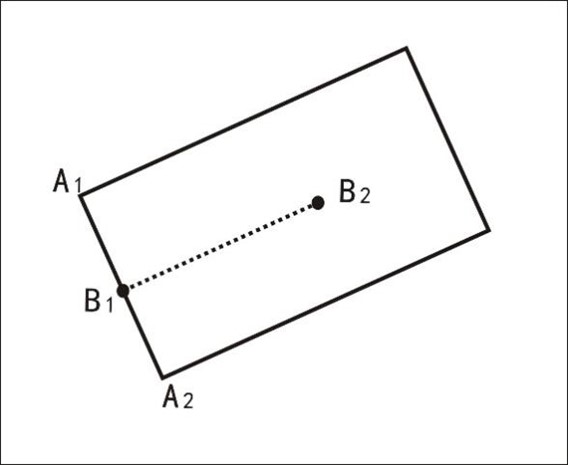
\includegraphics[scale=0.9]{6.jpg}
    \caption{交点坐标的计算}
\end{figure}
\noindent 得到直线$A$、$B$的方程为:
\begin{equation}
    l_{A}: \frac{\left(x-a_{1}\right)}{\left(a_{2}-a_{1}\right)}=\frac{\left(y-a_{3}\right)}{\left(a_{4}-, a_{4}\right)}
\end{equation}
\begin{equation}
    l_{B}: \frac{\left(x-b_{1}\right)}{\left(b_{2}-b_{1}\right)}=\frac{\left(y-b_{3}\right)}{\left(b_{4}-, b_{4}\right)}
\end{equation}
联立方程:
\begin{equation*}
    \left\{\begin{aligned}
        \frac{\left(x-a_{1}\right)}{\left(a_{2}-a_{1}\right)}=\frac{\left(y-a_{3}\right)}{\left(a_{4}-, a_{4}\right)} \\
        \frac{\left(x-b_{1}\right)}{\left(b_{2}-b_{1}\right)}=\frac{\left(y-b_{3}\right)}{\left(b_{4}-, b_{4}\right)}
    \end{aligned}\right.
\end{equation*}
将相关点的坐标带入求解即可得交点坐标。这里设边框A的左顶点,边框A与车道线B、边框A与车道线C、边框A与障碍物D左侧交点分别为:$H_1,H_2,H_3,H_4$。

\noindent 所以无人车调头之后的最佳调头结束点为:
\begin{equation*}
    Z_{1}=\frac{H_{1}+H_{2}}{2} ; \quad Z_{2}=\frac{H_{2}+H_{3}}{2} ; \quad Z_{3}=\frac{H_{3}+H_{4}}{2}
\end{equation*}

\noindent 同理可求出其它交点坐标,这里设起点坐标、第一段与第二段的交点坐标分别为:$X_1,X_2$;

\noindent 第二段和第三段的交点坐标有三个,分别与调头结束点相对应设为:
$Y_1,Y_2,Y_3$。

\subsubsection{行车轨迹}
\noindent 由以上可知,无人车的驾驶轨迹为:

\noindent 路线1:$X_1\rightarrow X_2\rightarrow Y_1\rightarrow Z_1$,此时轨迹长度为$l_1$;

\noindent 路线2:$X_1\rightarrow X_2\rightarrow Y_2\rightarrow Z_2$,此时轨迹长度为$l_2$;

\noindent 路线3:$X_1\rightarrow X_2\rightarrow Y_3\rightarrow Z_3$,此时轨迹长度为$l_3$;
\begin{figure}[H]
    \centering
    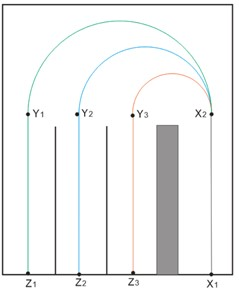
\includegraphics[scale=0.9]{7.jpg}
    \caption{多车道调头轨迹示意图}
\end{figure}

\subsubsection{数学模型的建立}
设无人车在轨迹中某一点的位置为$x_0$,时刻为$t_0$,设置自动驾驶调头所用总时间为$t$,在某一时刻障碍物与无人车的距离为$d_0$,在某一时刻轨迹点的曲率为$k_0$,于是构建单目标优化模型\cite{余卓平2017无人车运动规划算法综述}。

决策变量为:$x_0$

目标函数为:$mint=L/\bar{v}$ , $L=l_1$、$l_2$、$l_3$,$\bar{v}$̅为行驶时的平均速度。

约束条件为:

设置汽车的加速度为$a$,由于任何点的加速度不得高于最大油门加速度,不得低于极限刹车减速度,所以得到:
\begin{equation}
    -5 \leq a \leq 3
\end{equation}

车辆与障碍物至少保留一个最小安全距离,一般不小于 30cm;
\begin{equation}
    d_0 \geq  30
\end{equation}

方向盘与前轮转动角的传动比为 16:1,方向盘最大转角 $470^{\circ}$ 方向盘最大
转速为 $400^{\circ}$/s; 设置前轮的转动角为 $\alpha$ ,转速为 $\varepsilon$ ,所以有:
\begin{equation}
    \alpha  =\frac{470}{16}
\end{equation}
\begin{equation}
    \varepsilon  <\frac{400}{16}
\end{equation}
车轮轴距 L=2. 8m,则有:
\begin{equation}
    R=\frac{L}{\tan \alpha}
\end{equation}

由以上可知曲率半径应满足:
\begin{equation}
    r>4.878
\end{equation}

综上得:
\begin{equation*}
    \left\{\begin{aligned}{c}
        -5 \leqslant a \leqslant 3 ;                        \\
        d_{0} \geq 30                                       \\
        \alpha=\frac{470}{16}, \varepsilon<\frac{400}{16} ; \\
        R=\frac{L}{\tan \alpha}                             \\
        r>4.878
    \end{aligned}\right.
\end{equation*}

\subsubsection{求解结果}
由以上约束条件,将无人车调头过程分为三段,其中第二段和第三段为直行路段,第二段为转弯路段,这里是采用插值拟合的方法,先讨论出合适的调头路线,再进行建立目标优化模型,得到无人车的调头轨迹为:
\begin{figure}[H]
    \centering
    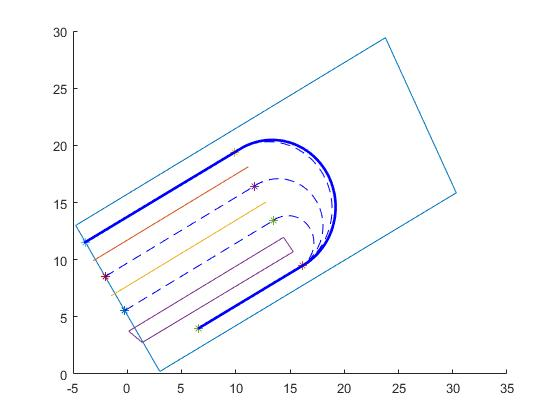
\includegraphics[scale=0.5]{8.jpg}
    \caption{无人车调头轨迹图}
\end{figure}

\subsection{倒车型}
\subsubsection{转弯半径的确定}
这里需要求解无人车在调头时需要进行调头的情况,则在这里讨论无人车刚好不需要进行调头,此时的转弯半径r变为最小半径,有:
\begin{equation}
    r = 4.878
\end{equation}

\subsubsection{无人车理想调头路线过程分析}
无人车的调头路线分为三段,第一段为直行,第二段为弧形(向左转180°即半个圆),第三段为直行。

第一段直行路线的起点即为无人车的初始位置,第一段和第二段的交点仍然为过起点且平行于障碍物D的直线与障碍物D横向直线的交点;然后无人车向左转弯180°,转弯半径$r$=4.478m到达第二段与第三段的交点;然后车辆沿着与车道线平行的方向行驶,到达调头区域,调头完成。

\subsubsection{关键坐标的计算}
第一段的起点坐标仍然为 $X_{1}$
第二段与第三段的交点坐标 $Y_{4}$ 为求解过程如下:

记
\begin{equation*}
    tan\alpha_{1}=k_{l_{D_{2} D_{3}}} \quad \alpha_{2}=\pi-\alpha_{1}
\end{equation*}
\begin{equation*}
    Y_{4}\left(x_{21}-2 r \cos \alpha_{2}, \quad x_{22}+2 r \sin \alpha_{2}\right)
\end{equation*}

同理可求得调头的终点,设为$Z_4$。

\subsubsection{驾驶轨迹}
此时无人车的驾驶轨迹为:
$X_{1} \rightarrow X_{2} \rightarrow Y_{4} \rightarrow Z_{4} ;$ 此时轨迹长度为 $l_{4}$。
\begin{figure}[h]
    \centering
    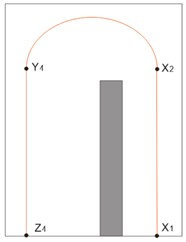
\includegraphics[scale=0.9]{9.jpg}
    \caption{倒车型调头轨迹示意图}
\end{figure}

\subsubsection{模型建立}
该模型与第一问的模型基本一致,唯一改变的为曲率半径,则目标函数仍然为:

目标函数为:
\begin{equation}
    \min t=\frac{L}{\bar{v}}
\end{equation}
\begin{equation}
    L=l_{4}
\end{equation}

约束条件为:
\begin{equation*}
    \left\{\begin{array}{c}
        -5 \leqslant a \leqslant 3 ;                        \\
        d_{0} \geq 30                                       \\
        \alpha<\frac{470}{16}, \varepsilon<\frac{400}{16} ; \\
        R=\frac{L}{\tan \alpha}                             \\
        r=4.878
    \end{array}\right.
\end{equation*}

\subsubsection{求解结果}
由以上模型求解得到的无人车轨迹为:
\begin{figure}[h]
    \centering
    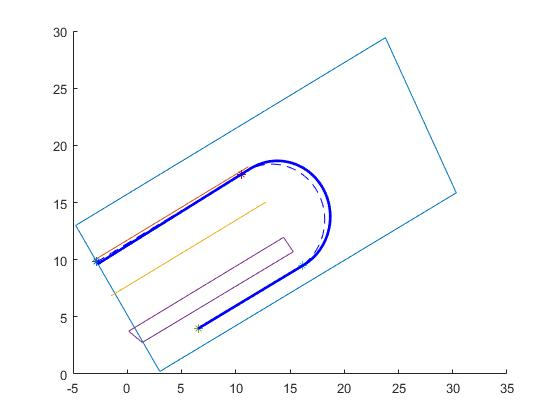
\includegraphics[scale=0.4]{10.jpg}
    \caption{无人车调头轨迹}
\end{figure}

\subsection{静止障碍物型}
如果道路上还存在其它静止障碍物时,分别对仅存在障碍物F、仅存在障碍物G、或二者都存在时这三种情况作分析。

\subsubsection{仅存在F时}
\begin{figure}[h]
    \centering
    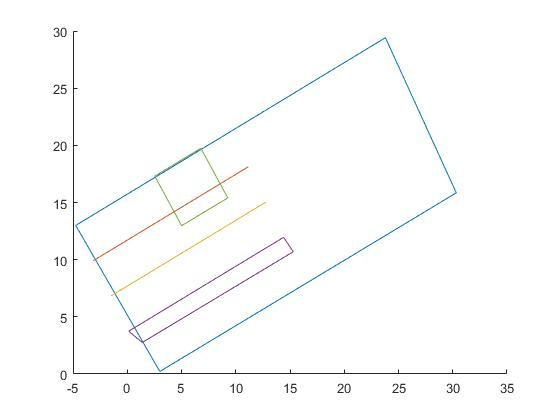
\includegraphics[scale=0.4]{11.jpg}
    \caption{无人车调头轨迹}
\end{figure}

\paragraph{无人车理想调头路线过程分析}
从图12可以看出,障碍物F占据了整个1车道和半个2车道,因此对无人车的路线规划时,只考虑从3车道通过。

同样,对于无人车的路线依然分为三段,且第一段直行路线不变,而对第二段的调头和第三段的路线作改变。第二段调头部分再分为三个小部分,如图中的\circled{2}\circled{3}\circled{4}所示,第三段部分即为\circled{5},则根据\circled{4}的终点来确定其具体路线。

\begin{figure}[h]
    \centering
    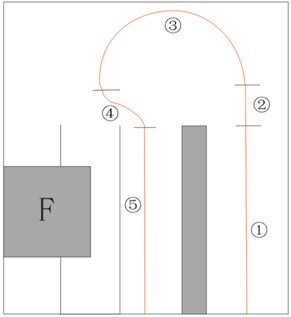
\includegraphics[scale=0.8]{12.jpg}
    \caption{无人车调头轨迹}
\end{figure}

\paragraph{路线的确定}
\begin{enumerate}[\indent 路线1:]
    \item 与前面一致保持不变;
    \item 设置这条路线为直线,目的是拉长距离方便进行转弯调头,路线的长度则根据\circled{1}的长度和场地大小设定一个参数值,只要保证后续路线符合约束条件即可。
    \item 根据曲率求出允许的最小半径,以该半径长度作圆为路线,行驶至一定距离后进入路线\circled{4}。
    \item 为了使无人车从调头处顺利进入车道,需要将方向盘回调,而这段回调的路线则是右转弯的,因此曲率取负数同样作圆即可。
    \item 当路线\circled{4}行驶后,只要从其终点,平行于车道行驶至调头区域边界线,则完成整个调头路线。
\end{enumerate}

\paragraph{关键坐标的计算}
\noindent 第一段的起点坐标仍然为 $X_{1}$

\noindent 第一段和第二段的交点坐标为 $X_{2}\left(x_{2}, y_{2}\right)$

\noindent 第二段与第三段的交点坐标 $Y_{5}\left(x_{5}, y_{5}\right)$

\noindent 第二段中路线(2)与路线(3)、路线(3)与路线(4)的交点坐标分别为 $Y_{5}^{\prime}\left(x_{51}, y_{51}\right), Y_{5}^{\prime \prime}$,$\left(x_{52}, y_{52}\right)$

\noindent 设路线(2)、路线(3)、路线(4)的长度分别为 $L_{1} 、 L_{2} 、 L_{3}$, 则有:
\begin{equation}
    L_{1}=\sqrt{\left(x_{51}-x_{21}\right)^{2}+\left(y_{51}-y_{21}\right)^{2}}
\end{equation}
\begin{equation}
    L_{2}=2 r \cdot \arcsin \left(\frac{\sqrt{\left(x_{52}-x_{21}\right)^{2}+\left(y_{52}-y_{21}\right)^{2}}}{2 r}\right)
\end{equation}
\begin{equation}
    L_{3}=2 r \cdot \arcsin \left(\frac{\sqrt{\left(x_{5}-x_{21}\right)^{2}+\left(y_{5}-y_{21}\right)^{2}}}{2 r}\right)
\end{equation}
\noindent 过点 $Y_{5}\left(x_{5}, y_{5}\right)$ 作垂直 $\mathrm{A}$ 边界的线,即可求得调头的终点,设为 $Z_{5}$ 。

\paragraph{驾驶轨迹}
\noindent 此时无人车的驾驶轨迹为:

\noindent $X_{1}$ $\rightarrow $ $X_{2}$ $\rightarrow $ $Y_{5}^{\prime}$ $\rightarrow $ $Y_{5}^{\prime \prime}$ $\rightarrow $ $Z_{5}$ ;此时轨迹长度为$l_5$

\paragraph{求解结果}
\begin{figure}[H]
    \centering
    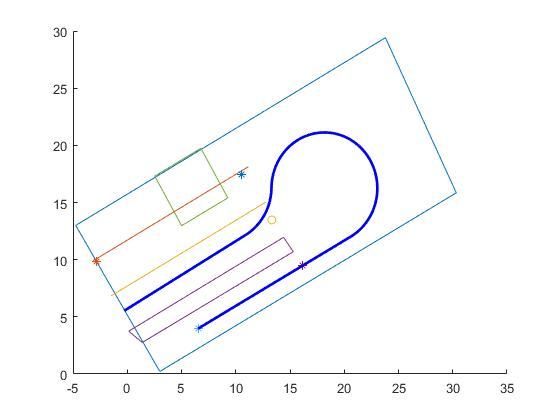
\includegraphics[scale=0.5]{13.jpg}
    \caption{仅存在F时无人车轨迹图}
\end{figure}

\subsubsection{仅存在障碍物G}
\begin{figure}[h]
    \centering
    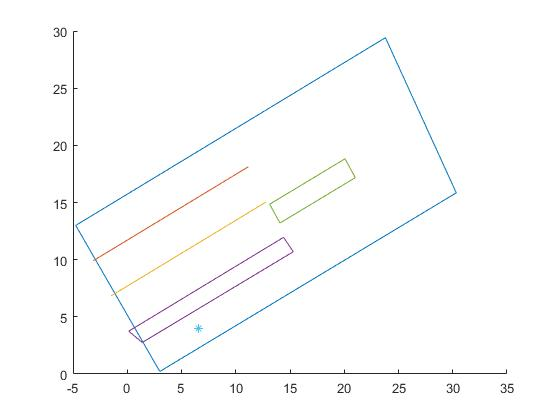
\includegraphics[scale=0.5]{14.jpg}
    \caption{仅存在G时无人车轨迹图}
\end{figure}

\paragraph{无人车理想调头路线过程分析}
从图15可以看出,障碍物G位于3车道的入口处,且几乎将车道完全阻挡,因此考虑无人车从1车道和2车道通过。
对于无人车的路线依然分为三段,第一段直行路线不变,而对第二段的调头和第三段的路线作改变。由于无人车可以从1车道或者2车道通过,所以当通过第一段后,设定两条路线分别从两车道行驶,即图中的路线\circled{1}和路线\circled{2}。
\begin{figure}[h]
    \centering
    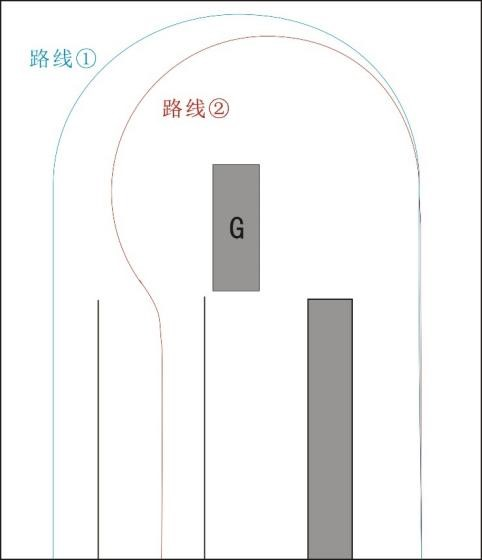
\includegraphics[scale=0.9]{15.jpg}
    \caption{仅存在G时的路线示意图}
\end{figure}

\paragraph{路线的确定}
\begin{enumerate}[\indent 第1段:]
    \item 与前面一致保持不变;
    \item 由于障碍物的存在,路线①和路线②都需要绕开其而做一个掉头。
          在路线\circled{1}中,为了顺利地进入1车道,掉头所需的半径则应该增大,由于最低的曲率半径为4.878m,通过逐步增大半径进行路线测试,最终设定其掉头半径为5.5m。在路线\circled{2}中,行驶路线与上一问中仅存在G时的路线相似,不同之处就是在于更改了路线长度的参数值。
    \item 当第二段路线行驶至车道中心附近,在保证不压车道线的情况下,平行于车道线行驶至掉头区域边界线即可。
\end{enumerate}

\paragraph{关键坐标的计算}
\noindent 第一段的起点坐标仍然为 $X_{1}$

\noindent 第一段和第二段的交点坐标为 $X_{2}\left(x_{2}, y_{2}\right)$

\noindent 路线\circled{1}中:

\noindent 第二段与第三段的交点坐标 $Y_{6}\left(x_{61}, y_{61}\right)$

\noindent 第三段与边界线的交点坐标为 $Z_{61}\left(x_{62}, y_{62}\right)$

\noindent 路线\circled{2}中:

\noindent 与上一问中仅存在 $\mathrm{F}$ 时类似,只是交点坐标不同;

\noindent 第二段中有交点坐标分别为 $Y_{6}^{\prime}\left(x_{63}, y_{63}\right) 、 Y_{6}^{\prime \prime}\left(x_{64}, y_{64}\right)$

\noindent 设第二段中三小段的长度分别为 $L_{1}^{\prime}, L_{2}^{\prime}, L_{3}^{\prime}$, 则有:
\begin{equation}
    L_{1}^{\prime}=\sqrt{\left(x_{63}-x_{21}\right)^{2}+\left(y_{63}-y_{21}\right)^{2}}
\end{equation}

\begin{equation}
    L_{2}^{\prime}=2 r \cdot \arcsin \left(\frac{\sqrt{\left(x_{64}-x_{21}\right)^{2}+\left(y_{64}-y_{21}\right)^{2}}}{2 r}\right)
\end{equation}

\begin{equation}
    L_{3}^{\prime}=2 r \cdot \arcsin \left(\frac{\sqrt{\left(x_{62}-x_{21}\right)^{2}+\left(y_{62}-y_{21}\right)^{2}}}{2 r}\right)
\end{equation}

\paragraph{驾驶轨迹}
此时无人车的驾驶轨迹为:

路线\circled{1}: $X_{1} \rightarrow X_{2} \rightarrow Y_{6} \rightarrow Z_{61} $; 此时轨迹长度为 $l_6$

路线\circled{2}: $X_{1} \rightarrow X_{2} \rightarrow Y_{6}^{\prime} \rightarrow Y_{6}^{\prime \prime} \rightarrow Y_{62} \rightarrow Z_{62} $此时轨迹长度为 $l_{6}^{\prime}$

\paragraph{求解结果}
路线\circled{1}:
\begin{figure}[H]
    \centering
    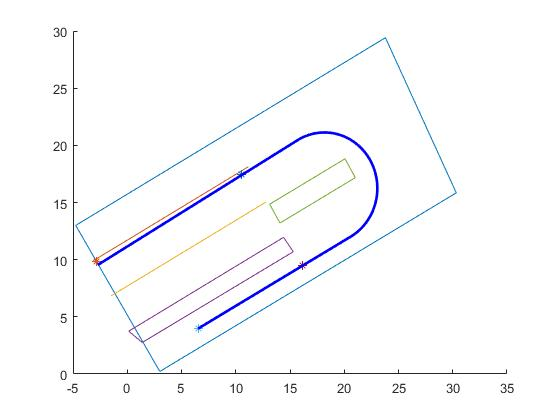
\includegraphics[scale=0.5]{16.jpg}
    \caption{仅存在G时无人车路线\textcircled{1}轨迹图}
\end{figure}

路线\circled{2}:
\begin{figure}[H]
    \centering
    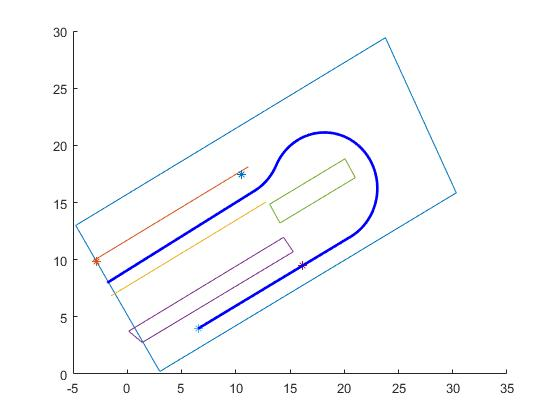
\includegraphics[scale=0.5]{17.jpg}
    \caption{仅存在G时无人车路线\textcircled{2}轨迹图}
\end{figure}

\subsubsection{F和G都存在时}
\begin{figure}[H]
    \centering
    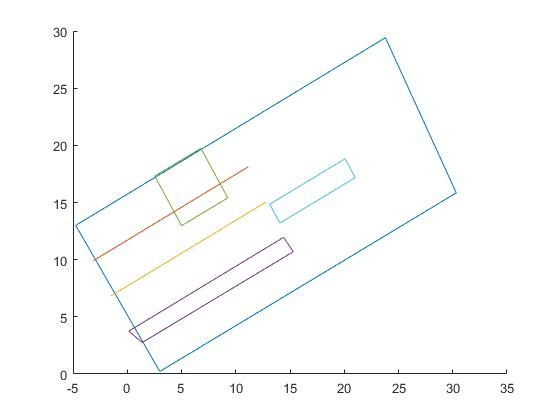
\includegraphics[scale=0.5]{18.jpg}
    \caption{F和G都存在时的路况示意图}
\end{figure}

\paragraph{无人车理想调头路线过程分析}
由于障碍物F完全占据1车道,障碍物G占据3车道入口,无人车的路线限制较大,因此设定无人车拐弯后,从2车道入口进入,再转向3车道直行。
\begin{figure}[H]
    \centering
    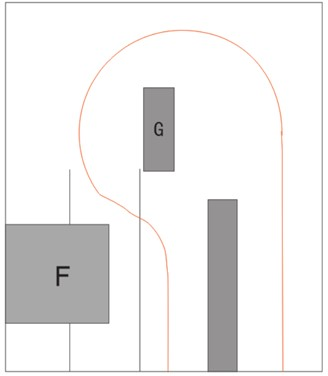
\includegraphics[scale=0.8]{19.jpg}
    \caption{F和G都存在时的路线示意图}
\end{figure}

\paragraph{路线的确定}
从图19的路线示意图可看出,路线情况同样与仅存在F时相似。
\begin{enumerate}[\indent 第1段:]
    \item 与前面一致保持不变;
    \item 由于障碍物G的存在,需绕过其而做一个转弯,该路线掉头中的左转弯部分与仅存在G时的路线②一致,当准备进入车道时,需要将方向盘打回,此时与仅存在F时的路线一致,不同之处在于打回的路线中应要注意障碍物F,为了保持安全距离,所转的弯会比较急。
    \item 当第二段路线行驶至3车道的中心线附近,在保证不压车道线的情况下,平行于车道线行驶至掉头区域边界线即可。
\end{enumerate}

\paragraph{关键坐标的计算}
\noindent 第一段的起点坐标仍然为 $X_{1}$

\noindent 第一段和第二段的交点坐标为 $X_{2}\left(x_{2}, y_{2}\right)$

\noindent 与上一问中仅存在 $\mathrm{F}$ 时类似,只是交点坐标不同;

\noindent 第二段中有交点坐标分别为 $Y_{7}^{\prime}\left(x_{71}, y_{71}\right), Y_{7}^{\prime \prime}\left(x_{72}, y_{72}\right)$

\noindent 设第二段中三小段的长度分别为 $L_{1}^{\prime \prime}, L_{2}^{\prime \prime} ,L_{3}^{\prime \prime}$, 则有:
\begin{equation}
    L_{1}^{\prime \prime}=\sqrt{\left(x_{71}-x_{2}\right)^{2}+\left(y_{71}-y_{2}\right)^{2}}
\end{equation}
\begin{equation}
    L_{2}^{\prime \prime}=2 r \cdot \arcsin \left(\frac{\sqrt{\left(x_{72}-x_{71}\right)^{2}+\left(y_{72}-y_{71}\right)^{2}}}{2 r}\right)
\end{equation}
\begin{equation}
    L_{3}^{\prime \prime}=2 r \cdot \arcsin \left(\frac{\sqrt{\left(x_{7}-x_{72}\right)^{2}+\left(y_{7}-y_{72}\right)^{2}}}{2 r}\right)
\end{equation}

\noindent 过点 $Y_{7}\left(x_{7}, y_{7}\right)$ 作垂直 $A$ 边界的线, 即可求得掉头的终点, 设为 $Z_{7}\left(x_{73}, y_{73}\right)$ 。

\paragraph{驾驶轨迹}
此时无人车的驾驶轨迹为:
$X_{1} \rightarrow X_{2} \rightarrow Y_{7}^{\prime} \rightarrow Y_{7}^{\prime \prime} \rightarrow Y_{7} \rightarrow Z_{7} ;$ 此时轨迹长度为 $l_{7}$

\paragraph{求解结果}
\begin{figure}[H]
    \centering
    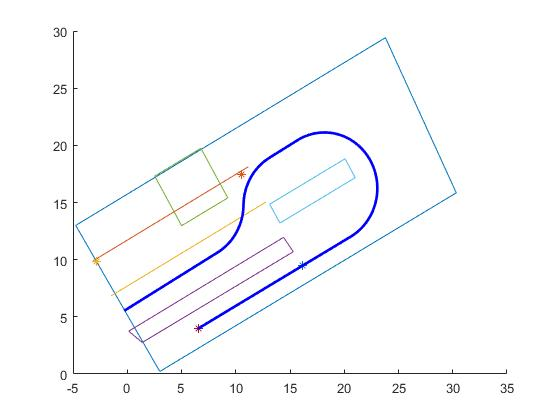
\includegraphics[scale=0.5]{20.jpg}
    \caption{F和G都存在的无人车轨迹图}
\end{figure}

\subsection{斑马线型}
\subsubsection{只存在斑马线时}
\begin{figure}[H]
    \centering
    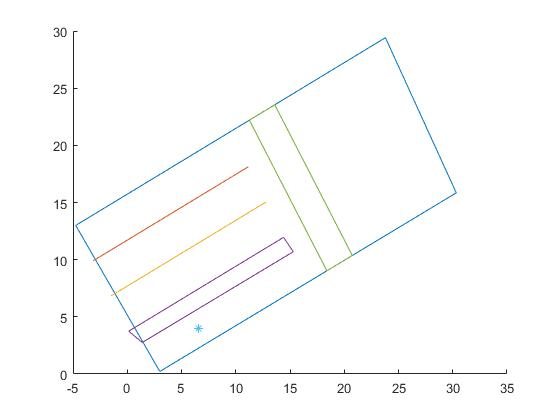
\includegraphics[scale=0.5]{21.jpg}
    \caption{存在斑马线时路况示意图}
\end{figure}

\paragraph{无人车调头路线分析}
题目需考虑到两种情况:不压斑马线和越过斑马线,分别在这两种情况下判断是否能完成掉头。设路线\circled{1}为不压斑马线,即从斑马线下方行驶;设路线\circled{2}为越过斑马线,即从斑马线上方行驶;

\paragraph{路线的确定}
路线\circled{1}:

将该路线分为5段,为了第3段的掉头能更加顺利,在启程时需要向右行驶一段距离,并保证车头在掉头前是朝向右边的。
\begin{enumerate}[\indent 第1段:]
    \item 无人车向右行驶一段距离。
    \item 为了与区域A保持安全距离,需将路线往回调,但车朝向仍向右。
    \item 保持直线向前行驶,到达掉头路口时即可准备掉头。
    \item 以最小曲率半径4.878作半圆为掉头的行驶路线。
    \item 平行于车道向前行驶至掉头区域边界线即可。
\end{enumerate}
\begin{figure}[H]
    \centering
    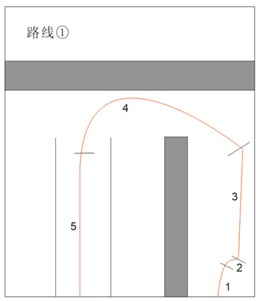
\includegraphics[scale=0.8]{22.jpg}
    \caption{不压斑马线无人车路线图}
\end{figure}

路线\circled{2}:

将该路线分为3段,与问题1的路线相似。
\begin{enumerate}[\indent 第1段:]
    \item 从出发点向前直行一定的距离。
    \item 以最小曲率直径作半圆为行驶路线,判断是否能越过斑马线,若不能越过则增加半径长度。
    \item 行驶至车道入口时,平行于车道向前行驶至掉头区域边界线即可。
\end{enumerate}
\begin{figure}[H]
    \centering
    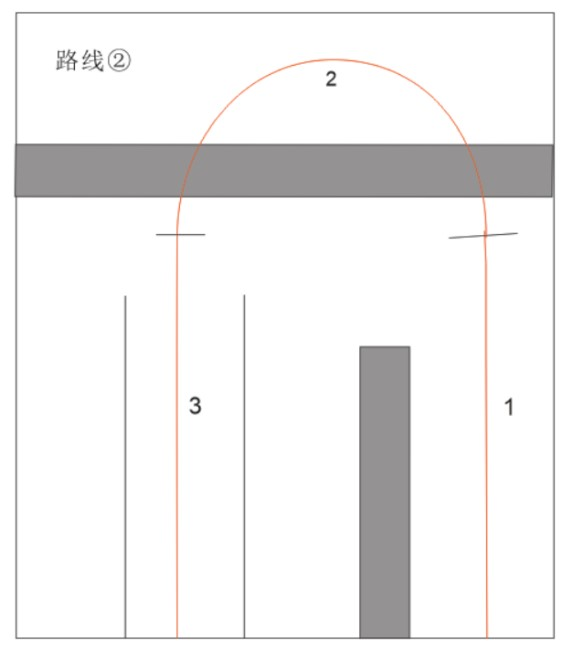
\includegraphics[scale=0.8]{23.jpg}
    \caption{越过斑马线无人车行驶路线图}
\end{figure}

\paragraph{求解结果}
路线\circled{1}——不压斑马线时:
\begin{figure}[H]
    \centering
    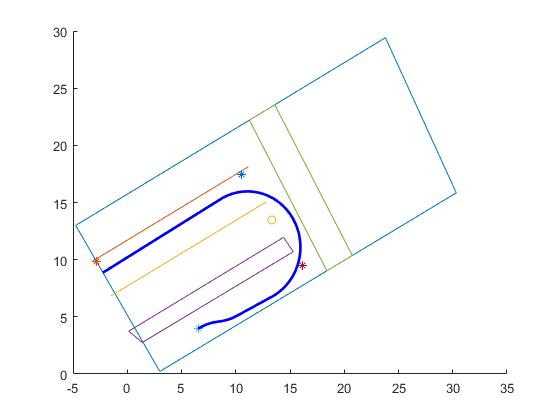
\includegraphics[scale=0.5]{24.jpg}
    \caption{无人车不压斑马线时轨迹图}
\end{figure}

路线\circled{2}——压斑马线时:
\begin{figure}[H]
    \centering
    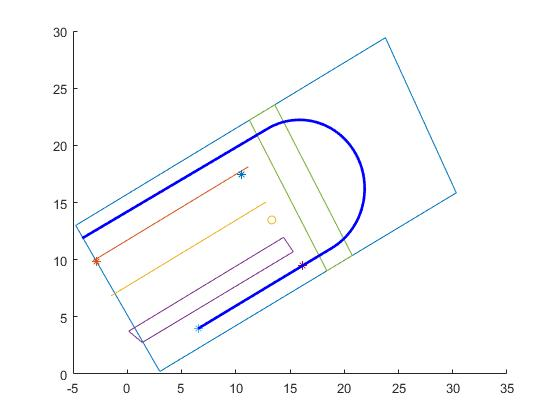
\includegraphics[scale=0.5]{25.jpg}
    \caption{无人车越过斑马线时轨迹图}
\end{figure}

\subsubsection{障碍物和斑马线同时存在时}
\begin{figure}[H]
    \centering
    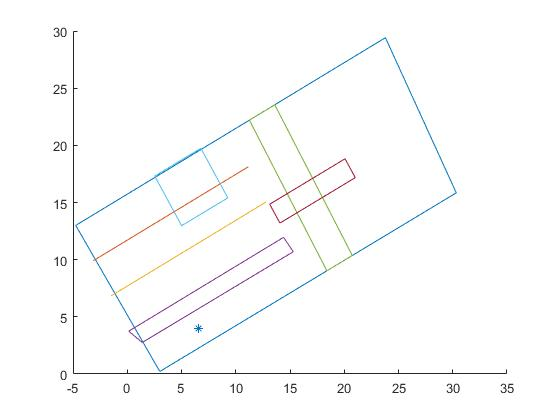
\includegraphics[scale=0.5]{26.jpg}
    \caption{斑马线和障碍物都存在时路况示意图}
\end{figure}

\paragraph{无人车调头路线分析}
同样也需考虑到两种情况:不压斑马线和越过斑马线,分别在这两种情况下判断是否能完成掉头。设路线\circled{1}为不压斑马线,即从斑马线下方行驶;设路线\circled{2}为越过斑马线,即从斑马线上方行驶;

\paragraph{路线的确定}
路线\circled{1}:
由于斑马线和障碍物的限制,若要从斑马线下过,则只能从障碍物G与隔离障碍物D间的路口通过。
\begin{enumerate}[\indent 第1段:]
    \item 无人车向前行驶一段距离。
    \item 到达掉头区域时,以最小曲率半径4.878作半圆为掉头的行驶路线。
    \item 平行于车道向前行驶至掉头区域边界线即可。
\end{enumerate}
\begin{figure}[H]
    \centering
    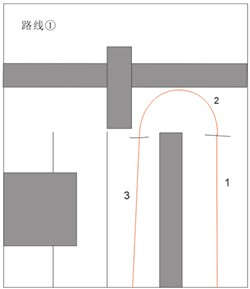
\includegraphics[scale=0.8]{27.jpg}
    \caption{不压斑马线无人车路线图}
\end{figure}

路线\circled{2}:
从图27的路线示意图可看出,路线情况与障碍物F与G同时存在时相似,不同之处在于多了一条斑马线,因此掉头的路线有所改变。
\begin{enumerate}[\indent 第1段:]
    \item 无人车直行一段距离。
    \item 以最小曲率半径4.8787m作圆为路线行驶越过斑马线。
    \item 越过斑马线后进入2车道,同时往3车道的方向行驶。
    \item 将无人车方向回调,以同样的半径作圆为路线。
    \item 平行于车道向前行驶至掉头区域边界线即可。
\end{enumerate}
\begin{figure}[H]
    \centering
    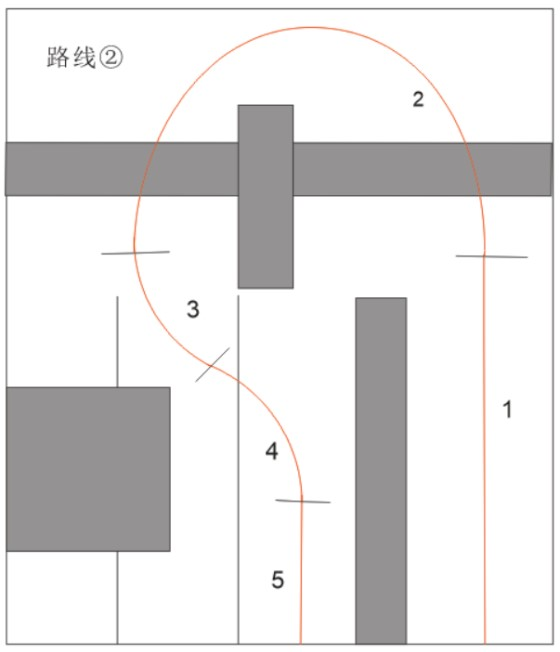
\includegraphics[scale=0.8]{28.jpg}
    \caption{越过斑马线无人车行驶路线图}
\end{figure}

\paragraph{求解结果}
路线\circled{1}——不压斑马线时:

通过matlab运行出的结果可以看出,这条路线无法顺利通过。
\begin{figure}[H]
    \centering
    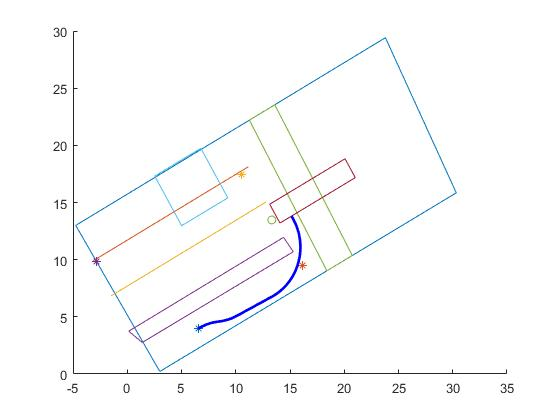
\includegraphics[scale=0.5]{29.jpg}
    \caption{无人车不压斑马线时轨迹图}
\end{figure}

路线\circled{2}——越过斑马线时:
\begin{figure}[H]
    \centering
    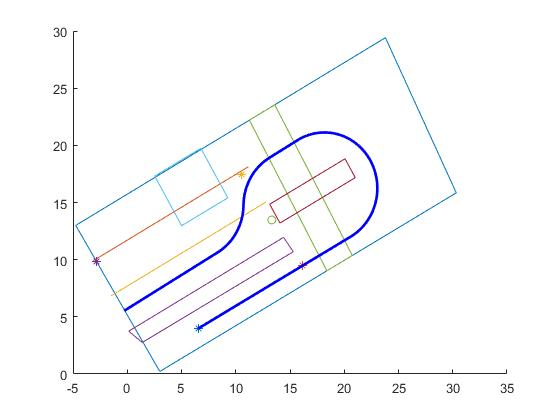
\includegraphics[scale=0.5]{30.jpg}
    \caption{无人车越过斑马线时轨迹图}
\end{figure}

\subsection{动态规划型}
针对问题5和问题6,采用动态路径规划避障的算法来求解。\cite{周慧子2017面向自动驾驶的动态路径规划避障算法}

\subsubsection{动态路径规划技术}
动态路径规划技术主要分为两大类: 第一类是全局路径规划,它是根据先验环境模型找出从起点到终点中符合条件的最优或次优路径,涉及的根本问题是环境模型的表达和路径搜寻策略;第二类是局部路径规划,是指在未知或部分未知的环境下通过传感器获取周围环境信息,并使自动驾驶汽车自主获得一条无碰撞最优规划的路径,它侧重于考虑车辆当前局部环境信息。\cite{王富奎2018高动态环境下智能车局部路径规划研究} 

\subsubsection{动态路径规划避障算法}
本题提出的动态路径规划方法是在已知车辆初始状态信息(包括车辆的位置、车头方向等)的基础上,产生一条安全又舒适的行驶路线。在已知全局路线的情况下进行局部规划,全局路线通过车道级的高精度导航系统获取。全局路线可以由一组道路边缘的有序点组成。如图31所示,所用方法包括三个部分:基准线生成、候选路径生成和最优路径选择。

\begin{figure}[H]
    \centering
    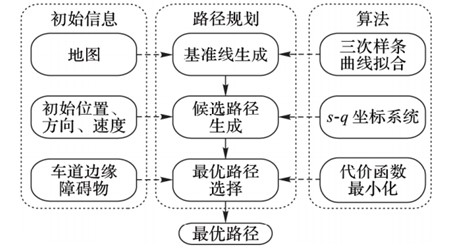
\includegraphics[scale=0.8]{31.jpg}
    \caption{动态路径规划算法流程}
\end{figure}

\newpage
\section{模型评价}
\subsection{路径规划与运动规划}
自动驾驶车辆中的调头问题需要给出车辆的轨迹路线,同时给出车辆沿该路径运动的速度信息,并且使车辆在整个运动过程中满足动力学约束及其它来自于外部环境和内部系统等约束条件。\cite{li2017nonlinear}

本文采用的是路径规划,与运动规划相比,路径规划仅仅只需生成满足空间约束条件的几何曲线,而如果采用运动规划,则会有以下难点:

(1)运动规划的过程复杂;

(2)通过运动规划生成的轨迹难以在后继控制模块中被有效跟踪;

(3)决策规划模块仅需生成路径而非轨迹,车辆实际运动速度暂时无法或无需决策。\cite{李柏2018自动驾驶车辆运动规划方法综述}

\subsection{模型优缺点}
本文解决问题的方法为插值拟合法,插值拟合法具有以下优点:

(1)求解路径的速度快;

(2)能够满足路径平滑性,可行性;

(3)方法简单。

但是插值拟合法由于采用特定类型的曲线函数描述行车路径,因此这一类方法无法充分发挥车辆的全部运动能录,因为车辆的动力学方程并不等价于插值拟合法中所使用的曲线函数。\cite{li2018balancing}。

\subsection{模型优化}
对于路径规划还可以采用其它方法如采样法、机器学习方法、最优控制方法等,其中最优控制方法能够有效地改进上述问题的不足,最优控制方法是采用建立微分方程组来描述车辆运动,同时在运动学微分方程的基础上补充必要的约束条件以及车辆行驶的性能指标式,这一方法将车辆运动规划问题描述为最优问题,具有客观、直接、统一、完备的优点。\cite{姚君延2018基于深度增强学习的路径规划算法研究}

\newpage

\section*{\centering{参考文献}}
\bibliographystyle{unsrt}
% unsrt 按照引用顺序
\bibliography{201847100213}
\thispagestyle{empty}
\newpage

\section*{\centering{附录}}
\begin{appendices}
    \section{问题一}
    \noindent \textcolor[rgb]{0,0,0}{\textbf{main.m}}
    \lstinputlisting[language=Matlab]{./code/main1.m}
    \section{问题二}
    \lstinputlisting[language=Matlab]{./code/main2.m}
    \section{问题二}
    \lstinputlisting[language=Matlab]{./code/main3_F.m}
    \lstinputlisting[language=Matlab]{./code/main3_FG.m}
    \lstinputlisting[language=Matlab]{./code/main3_G.m}
    \section{问题四}
    \lstinputlisting[language=Matlab]{./code/main4_E1.m}
    \lstinputlisting[language=Matlab]{./code/main4_E2.m}
    \lstinputlisting[language=Matlab]{./code/main4_EFG1.m}
    \lstinputlisting[language=Matlab]{./code/main4_EFG2.m}
    \section{ArcLength}
    \lstinputlisting[language=Matlab]{./code/Arc_Length.m}
    \section{drawArc}
    \lstinputlisting[language=Matlab]{./code/drawArc.m}
    \section{NextTrackPoint}
    \lstinputlisting[language=Matlab]{./code/Next_TrackPoint.m}
\end{appendices}
\end{document}
